\chapter{Results}
\label{ch:results}

\section{Hyperparameter selection}

A five-fold cross-validated grid search was performed with a fixed spherical harmonic degree at $L=26$. It searches over different combinations of $(\lambda,k)$ and then uses the aggregated five-fold cross-validated error to compare the different combinations. The lowest cross-validated error was found at $\lambda = 10^{-4}$ and $k=2$ with a reported minimum error of 41.27. This value is based on the aggregated $L^2$ prediction-error criterion described in \cref{ch:methodology}. 

\begin{figure}[H]
    \centering
    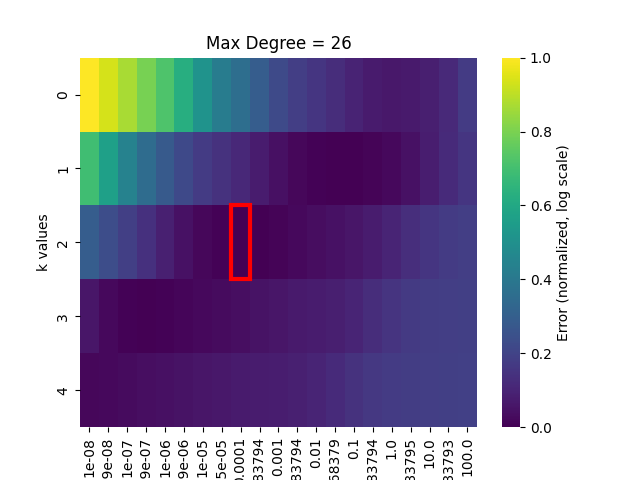
\includegraphics[width=0.72\textwidth]{figures/parameter_optimization_heatmap_L26.png}
    \caption{Five-fold cross-validated error surface over the regularisation strength $\lambda$ (x-axis) and Sobolev order $k$ (``k values'', y-axis) at fixed degree $L=26$. The selected minimum, $\lambda=10^{-4}$, $k=2$, is outlined in red.}
    \label{fig:heatmap}
\end{figure}

The heatmap shows how the cross-validated error changes with $\lambda$ and $k$ in \Cref{fig:heatmap}. The error decreases gradually when moving from $k=0$ (plain ridge-type regularisation) to $k=2$ (second-order Sobolev regularisation). This supports the idea that derivative-based regularisation is useful for the temperature reconstruction problem. $k=2$ provides stronger penalisation of high-degree and rough components, which helps reduce unnecessary high-frequency variation caused by noise. However, increasing $k$ too much can become overly restrictive. After $k=2$, the cross-validated error starts to increase again for larger $k$. This suggests that stronger smoothness penalties may begin to underfit genuine smaller-scale temperature variation. Therefore, the balance needs to be found where we cannot have either too little regularisation or too much. 

Although the heatmap does not show an extremely sharp minimum around $k=2$, the low-error region is relatively broad and shallow. This indicates that performance is not extremely sensitive to $k$ within the tested range, so the result aims to present some robustness choice of Sobolev order $k$. This finding is consistent with the predecessor dissertation that the second Sobolev seminorm could improve reconstruction compared with plain $L^2$ regularisation. Therefore, the current experiment provides an independent check using the temperature dataset and the current pipeline. Unless stated otherwise, the remaining experiments will use $L=26$, $\lambda=10^{-4}$, and $k=2$, which is selected from the grid search. The final configuration is then used in the subsequent conformal prediction experiments. 
 
\section{Standard versus adaptive coverage and width}
\label{sec:main-results}
\begin{table}[H]
\centering
\caption{Marginal coverage and mean interval width on the held-out test set ($n=351$, $\alpha=0.1$).}
\label{tab:main-coverage}
\begin{tabular}{lcc}
\toprule
Method & Marginal coverage & Mean interval width ($^\circ$C) \\
\midrule
Standard (non-adaptive) & 0.909 & 4.649 \\
Adaptive geodesic (proposed) & 0.937 & 4.592 \\
\bottomrule
\end{tabular}
\end{table}
The evaluation is performed on the held-out test set ($n=351$). The nominal conformal level ($\alpha=0.1$) corresponds to a target coverage of 90\%. The standard split conformal results show a marginal coverage of 90.9\% with a mean prediction interval width of $4.65^\circ\mathrm{C}$. In contrast, the proposed adaptive geodesic conformal results in a higher marginal coverage of 93.7\% with a mean prediction interval width of $4.59^\circ\mathrm{C}$ (\cref{tab:main-coverage}). Both approaches achieve the nominal 90\% coverage target on the held-out test set, which is consistent with the expected split-conformal coverage behaviour discussed in \cref{sec:cp-background} regardless of the spherical harmonic predictor used. However, the adaptive method provides higher coverage of 93.7\%, which is above the nominal 90\% target and slightly narrower mean prediction intervals. Besides, similar patterns can be seen across the different spherical harmonic degrees in the degree-robustness experiment \cref{tab:degree-robustness}. The variation across different $L$ values is also expected to align with finite-sample variation around the theoretical guarantee with $n_{cal}=351$. Overall marginal coverage alone is not the main reason for introducing the adaptive method. Since both methods already achieve approximately the desired overall coverage, the more important question is whether coverage remains reliable across locations with different prediction difficulties. Therefore, the next analysis focuses on conditional/difficulty-stratified coverage.
\begin{table}[H]
\centering
\caption{Conditional coverage and interval width by difficulty tertile (test set, $n=351$).}
\label{tab:tertile}
\begin{tabular}{lcccccc}
\toprule
Tertile & $n$ & $\overline{\hat\sigma}$ & $\overline{|e|}$ & Std.\ cov. & Adapt.\ cov. & Std.\ / Adapt.\ width \\
\midrule
Low difficulty & 118 & 0.310 & 0.366 & 1.000 & 0.915 & 4.649 / 1.481 \\
Medium difficulty & 117 & 0.815 & 0.820 & 0.957 & 0.949 & 4.649 / 3.893 \\
High difficulty & 116 & 1.770 & 1.904 & 0.767 & 0.948 & 4.649 / 8.460 \\
\bottomrule
\end{tabular}
\end{table}
The test set is split into three equal-frequency tertiles based on estimated local difficulty $\hat\sigma(x)$ to examine conditional/difficulty-dependent coverage, which cannot be seen from the overall marginal coverage (\cref{tab:tertile}). The standard method provides excessive coverage in the easiest tertile (100\% coverage above the 90\% target, with a fixed $4.65^\circ\mathrm{C}$ interval), while it demonstrates a sharp drop in the hardest tertile (76.7\% coverage, a 13.3 percentage-point gap below the target). These results show that the standard method does not maintain coverage consistently across different difficulty levels. In contrast, the adaptive method keeps coverage within a narrow $91$-$95\%$ range for all three difficulty groups, while obtaining a much narrower mean interval width of $1.48^\circ\mathrm{C}$ in the easiest tertile and a wider width of $8.46^\circ\mathrm{C}$ in the hardest tertile. This reflects that easier locations receive narrower intervals, while more difficult locations with greater uncertainty receive wider intervals. The hardest tertile also has a higher mean absolute prediction error of $1.90^\circ\mathrm{C}$, compared with the easiest tertile of $0.37^\circ\mathrm{C}$. This result shows that the adaptive method is responding to differences in local prediction difficulty and gives more balanced coverage across difficulty levels with varying interval widths according to local difficulty.
\begin{figure}[H]
    \centering
    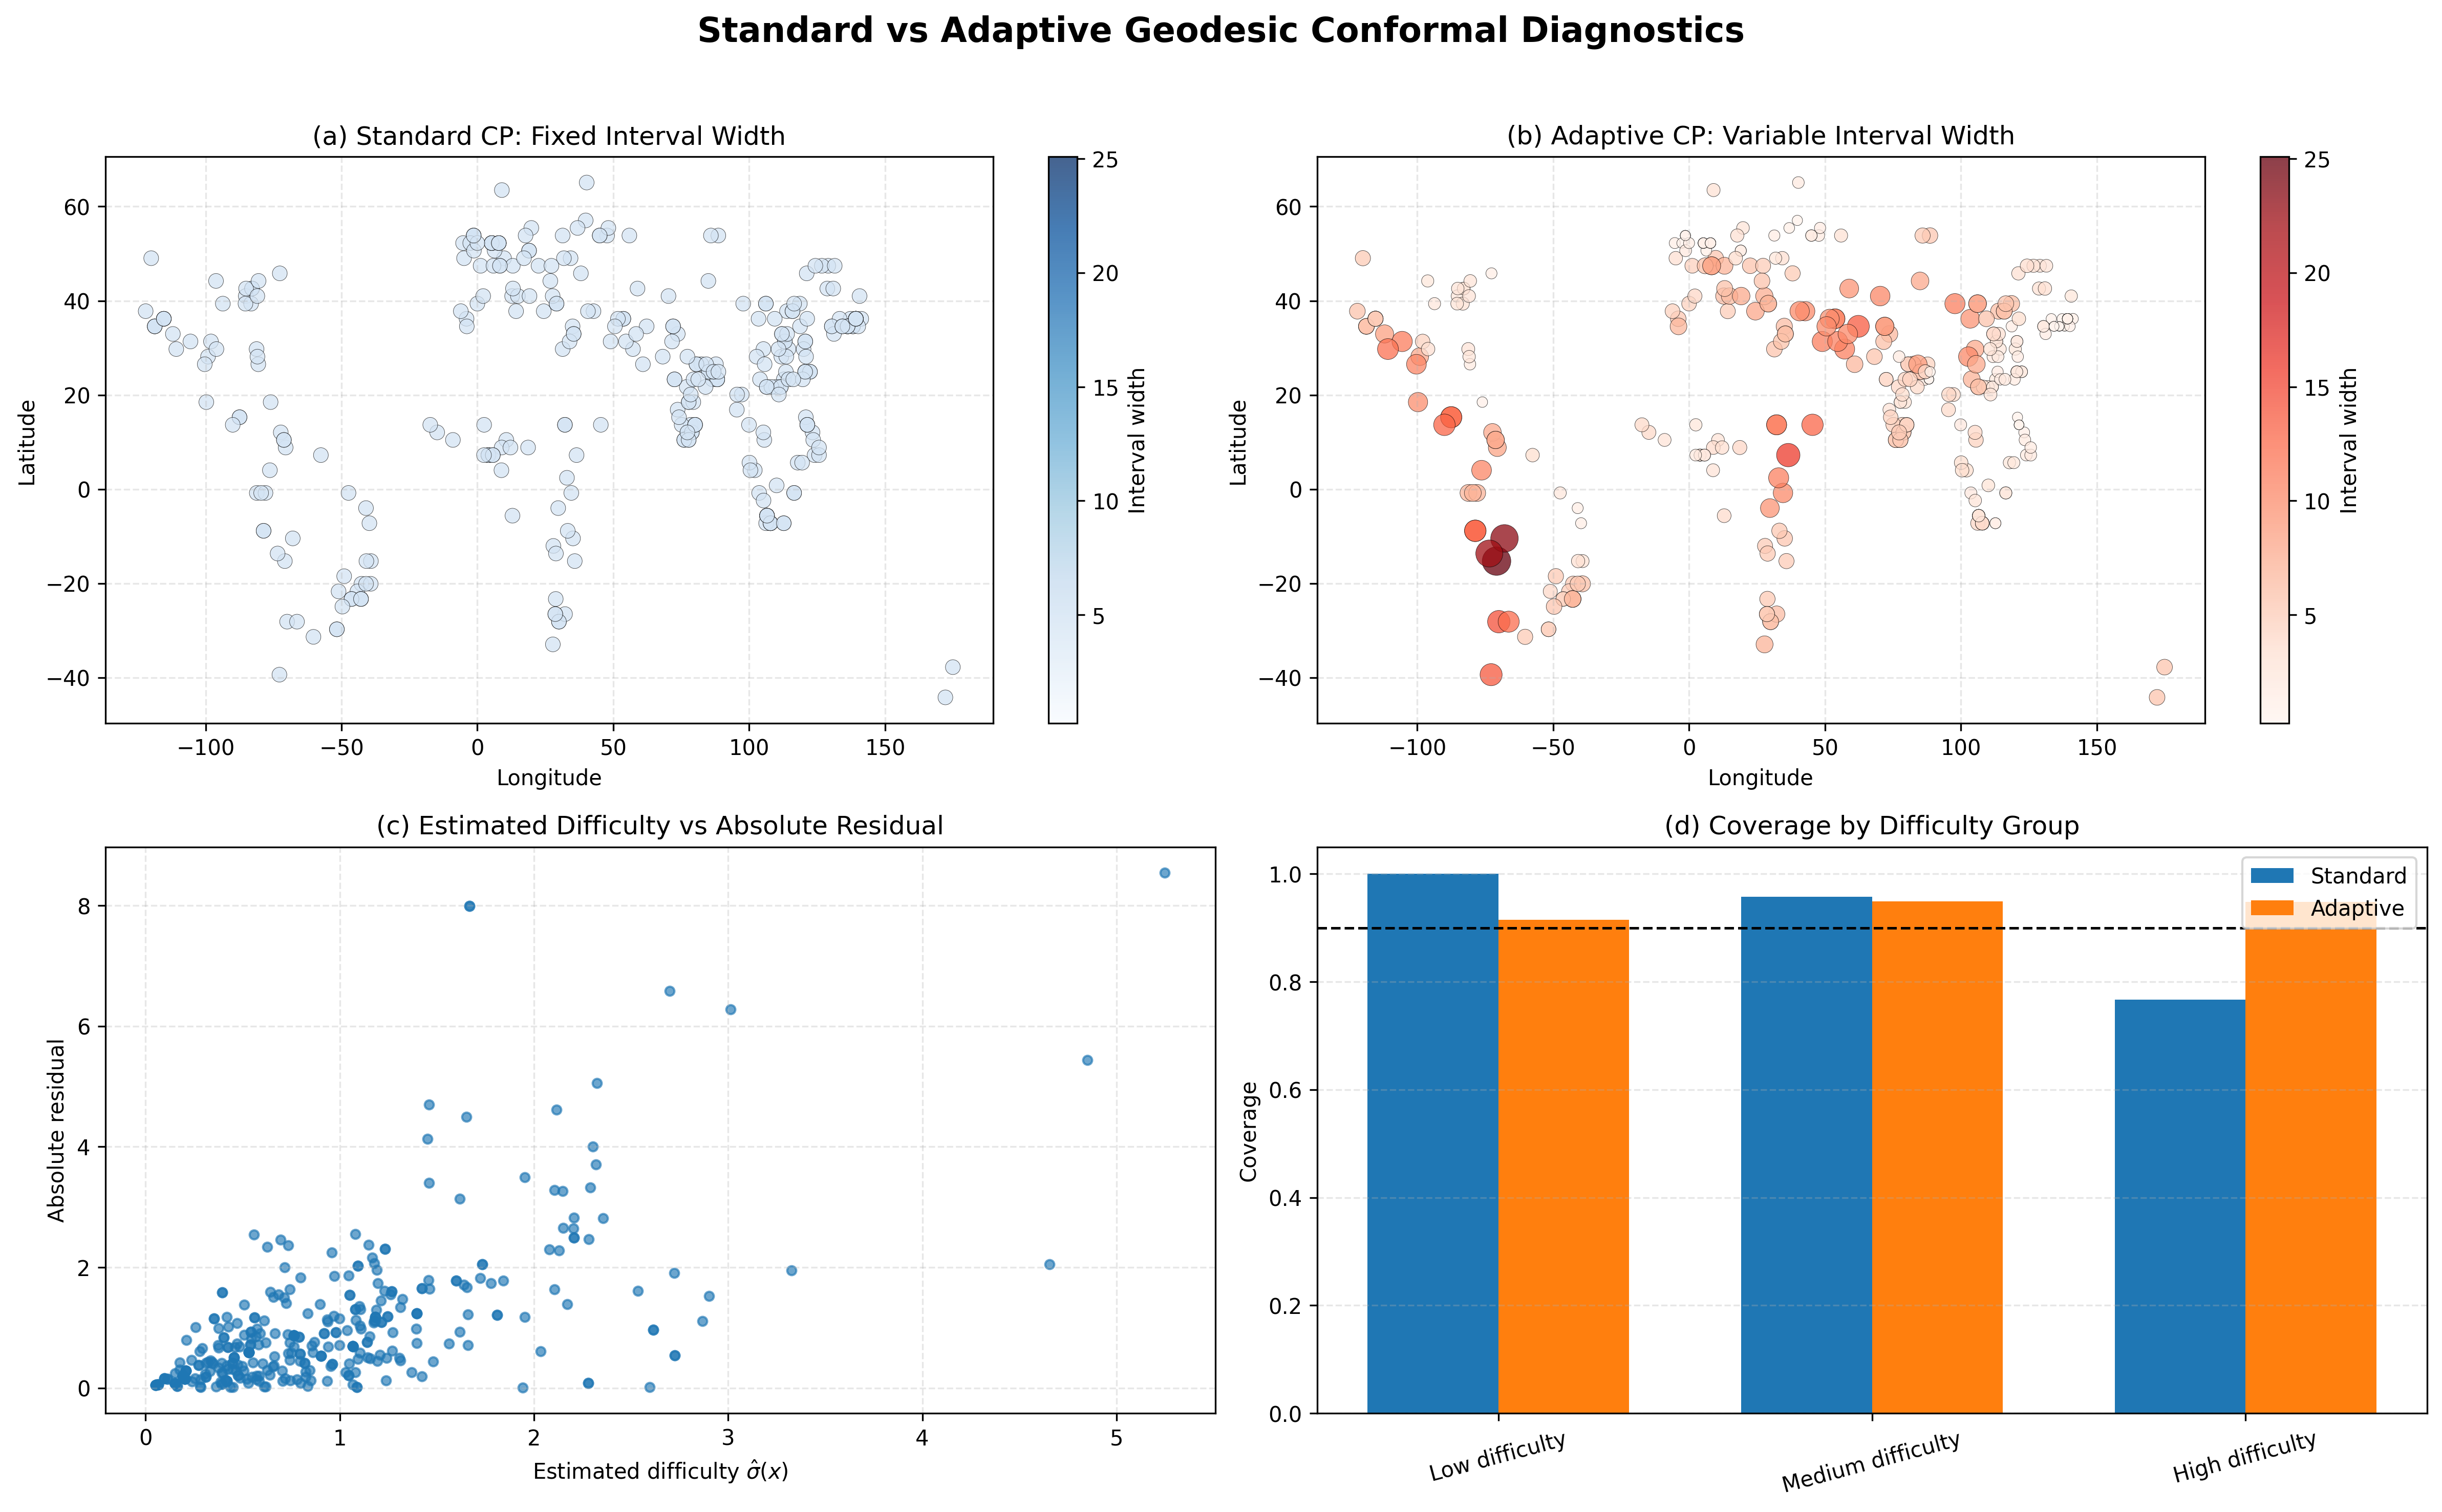
\includegraphics[width=\textwidth]{figures/standard_vs_adaptive_conformal_diagnostic.png}
    \caption{Standard versus adaptive geodesic conformal diagnostics on the test set. (a)/(b) Geographic distribution of interval width (marker size and colour) for the standard and adaptive methods. (c) Estimated difficulty $\hat\sigma(x)$ against true absolute residual. (d) Empirical coverage by difficulty tertile against the nominal $90\%$ target (dashed line).}
    \label{fig:main-diagnostic}
\end{figure}
\Cref{fig:main-diagnostic} presents the main result from both geographical and statistical perspectives. Panel (a) shows the spatial pattern of the standard conformal interval width, which is uniform across the spatial domain. Panel (b) shows that the adaptive method's interval widths vary across locations according to the estimated difficulty. Larger intervals are mainly found at high-difficulty locations, which are noticeably concentrated in western South America. Panel (c) shows a positive relationship between estimated difficulty $\hat\sigma(x)$ and the actual absolute prediction residual. Panel (d) gives the clearest single summary of the main result and visually demonstrates the difference in difficulty-stratified/conditional coverage: adaptive coverage (in orange) remains close to the 90\% target across all groups; standard coverage (in blue) varies between the groups.
\begin{figure}[H]
    \centering
        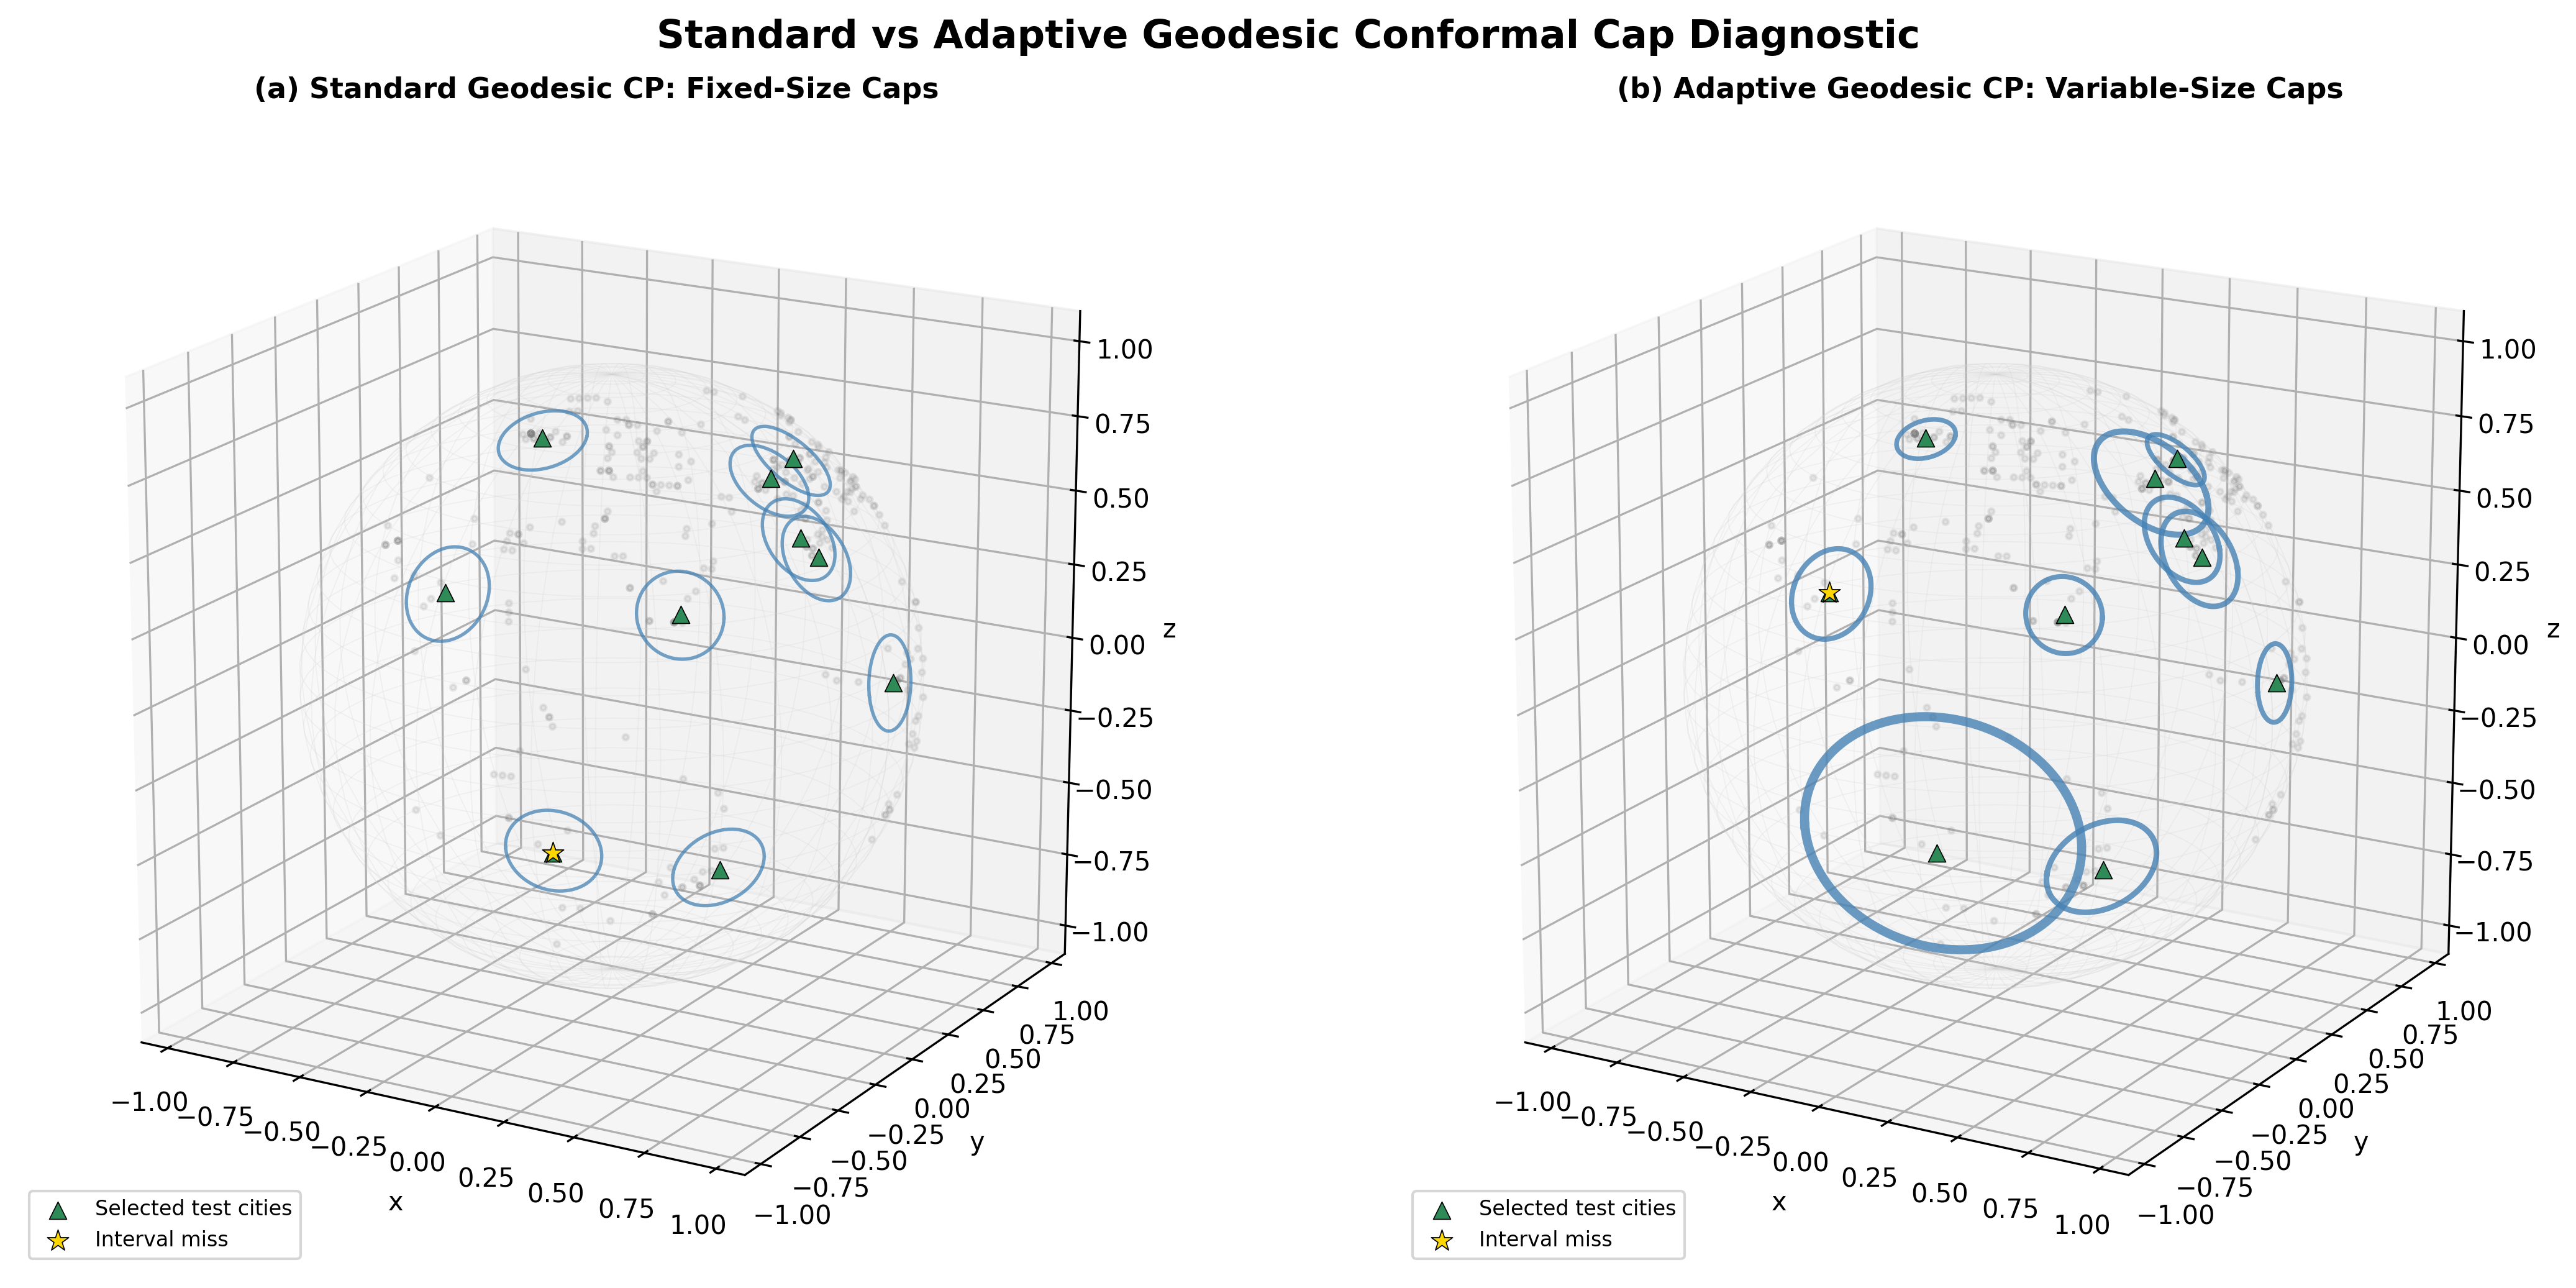
\includegraphics[width=\textwidth]{figures/standard_vs_adaptive_geodesic_caps.png}
    \caption{Illustrative fixed-size (standard, left) versus variable-size (adaptive, right) interval radii, drawn as circles on the input sphere for a representative subsample of test cities spanning the full difficulty range. Circle size is proportional to interval half-width; the gold star marks a coverage miss.}
    \label{fig:caps}
\end{figure}
\Cref{fig:caps} provides a geometric visualisation of the same adaptive uncertainty behaviour directly on the sphere. The standard conformal method uses the fixed-radius prediction caps, which do not change according to local difficulty. The adaptive method uses variable-radius caps, where larger caps are assigned to locations with higher estimated difficulty. The green triangles indicate the selected test cities, which are chosen to span the range of estimated prediction difficulty from low to high; the same locations are shown in both panels to allow a direct comparison between the standard and adaptive methods. The gold stars indicate test locations where the corresponding prediction cap does not contain the true value. In one example, the standard method's fixed and smaller cap does not cover the true value, while the adaptive method assigns a larger cap at the same location and successfully covers it. Conversely, another location is covered by the standard method but is missed by the adaptive method. These examples illustrate that adaptive conformal prediction does not eliminate individual misses, but instead reallocates interval width according to local prediction difficulty. The cap radii are visually rescaled rather than plotted using the raw values of $\hat q$ and $\hat q\hat\sigma(x)$, since these quantities are measured in temperature units, whereas the spherical cap radii are angular distances on the unit sphere. For visualisation, the adaptive interval widths are linearly mapped to spherical radii between $0.10$ and $0.45$, with smaller and larger radii corresponding to lower and higher estimated uncertainty, respectively. The standard method uses a single fixed visual radius, set to the median of the adaptive visual radii, to represent its constant interval width. The rescaling therefore preserves the relative differences in uncertainty while providing a meaningful geometric visualisation. Overall, the figure provides an intuitive geometric illustration of how adaptive interval widths respond to spatially varying prediction difficulty.

\section{Difficulty-estimator quality}
\begin{figure}[H]
    \centering
    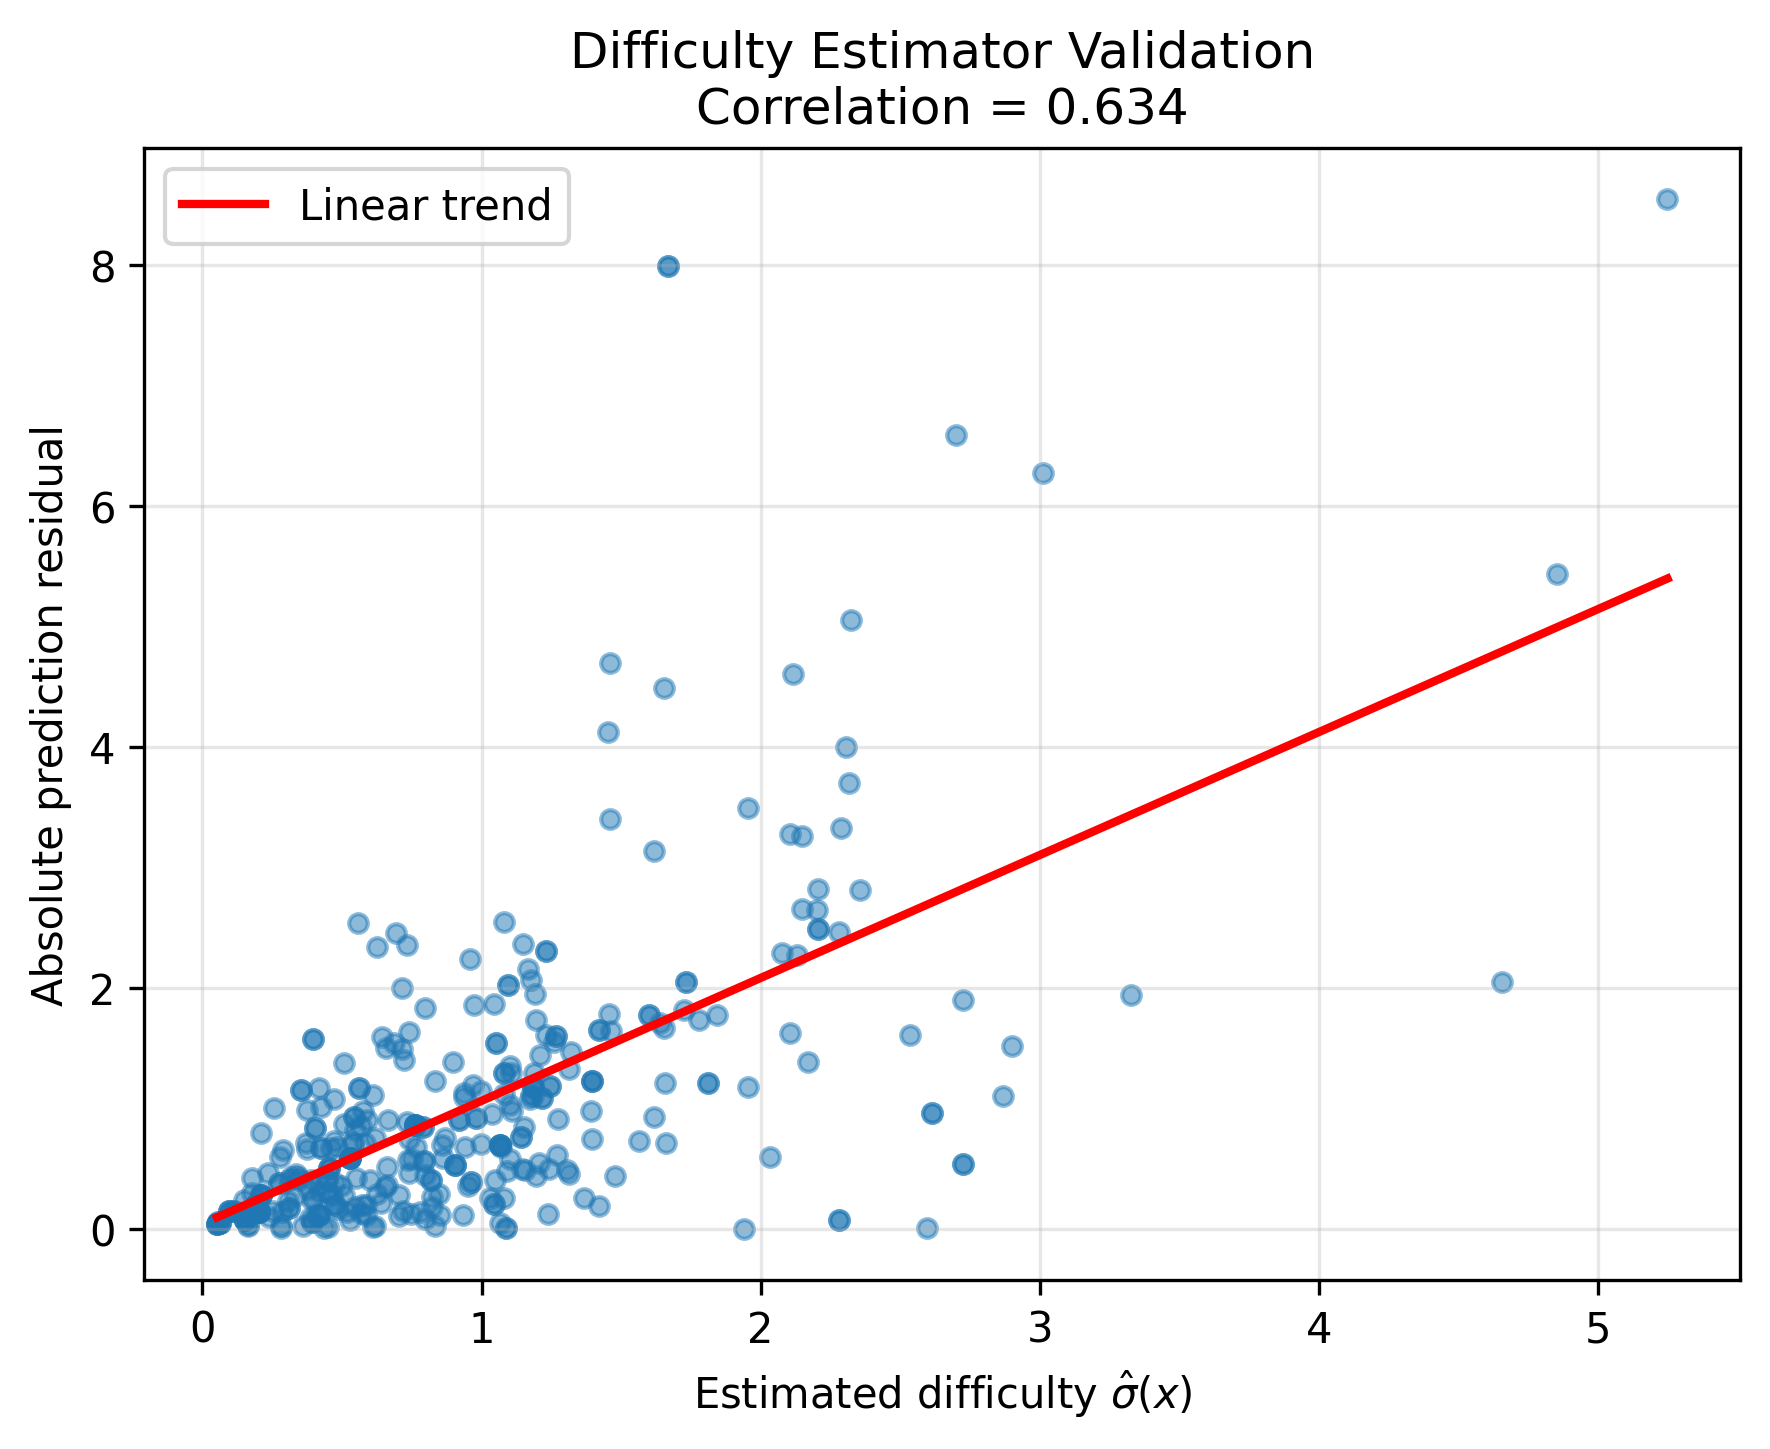
\includegraphics[width=0.65\textwidth]{figures/difficulty_validation.png}
    \caption{Estimated difficulty $\hat\sigma(x)$ against true absolute prediction residual on held-out data, with a linear trend line. Pearson $r=0.634$.}
    \label{fig:difficulty-validation}
\end{figure}
The Pearson correlation between the estimated difficulty $\hat\sigma(x)$ and the absolute prediction error on the held-out test set was $r=0.634$ (\cref{fig:difficulty-validation}). This indicates a clear positive relationship between the estimated local difficulty and the observed prediction error. Locations that are estimated to be more difficult generally tend to have larger prediction errors. The plot shows that $\hat\sigma(x)$ captures meaningful spatial variation in reconstruction difficulty. The current correlation result of $r=0.634$ is higher than the value reported by \citet{amirishahbazi2026} for their real-world IGRF-14 geomagnetic case study of $r=0.516$. Their experiments also found that correlations above approximately $0.3$ were associated with useful adaptive behaviour, however, this value should not be presented as a universal threshold. It should only be treated as an empirical reference from their experiments. 

With the current dataset, the result suggests that the geodesic $k$-nearest-neighbour residual estimator provides a useful measure of local reconstruction difficulty. Possible explanations for the difference from \citet{amirishahbazi2026}'s result are discussed in\cref{ch:discussion}. Correlation shows an empirical association but does not establish the physical cause of the relationship.

\section{Fine-grained conditional coverage}
\begin{table}[H]
\centering
\caption{Adaptive method conditional coverage across six equal-frequency difficulty bins (test set, $n=351$).}
\label{tab:sixbin}
\begin{tabular}{lccc}
\toprule
Bin & $n$ & Mean $\hat\sigma$ & Coverage \\
\midrule
1 (easiest) & 59 & 0.185 & 0.949 \\
2 & 59 & 0.435 & 0.881 \\
3 & 59 & 0.663 & 0.898 \\
4 & 58 & 0.969 & 1.000 \\
5 & 57 & 1.256 & 0.965 \\
6 (hardest) & 59 & 2.267 & 0.932 \\
\bottomrule
\end{tabular}
\end{table}
Instead of three difficulty tertiles, dividing the test set into six equal-frequency difficulty bins provides a more detailed assessment of how coverage changes across different levels of estimated difficulty and checks whether the adaptive method maintains stable coverage.  (\cref{tab:sixbin}). Coverage across the six bins ranges from $88.1\%$ to $100\%$, with a standard deviation of $0.0436$ and a worst-bin coverage of $88.1\%$. The worst bin is therefore $1.9$ percentage points below the nominal $90\%$ target. This indicates that the adaptive method maintains relatively stable coverage across the different levels, with no difficulty bin showing a very large departure from the target coverage. Thus, the adaptive method provides more consistent conditional coverage across locations with different difficulty levels, with its worst six-bin coverage of 88.1\% also being higher than the 76.7\% coverage observed in the worst tertile for the standard method (\cref{tab:tertile}). Overall, the six-bin analysis provides additional evidence that the adaptive method is not only achieving good marginal coverage but also maintaining relatively stable coverage across different difficulty levels.

\section{Robustness across spherical harmonic degree}
\begin{figure}[H]
    \centering
    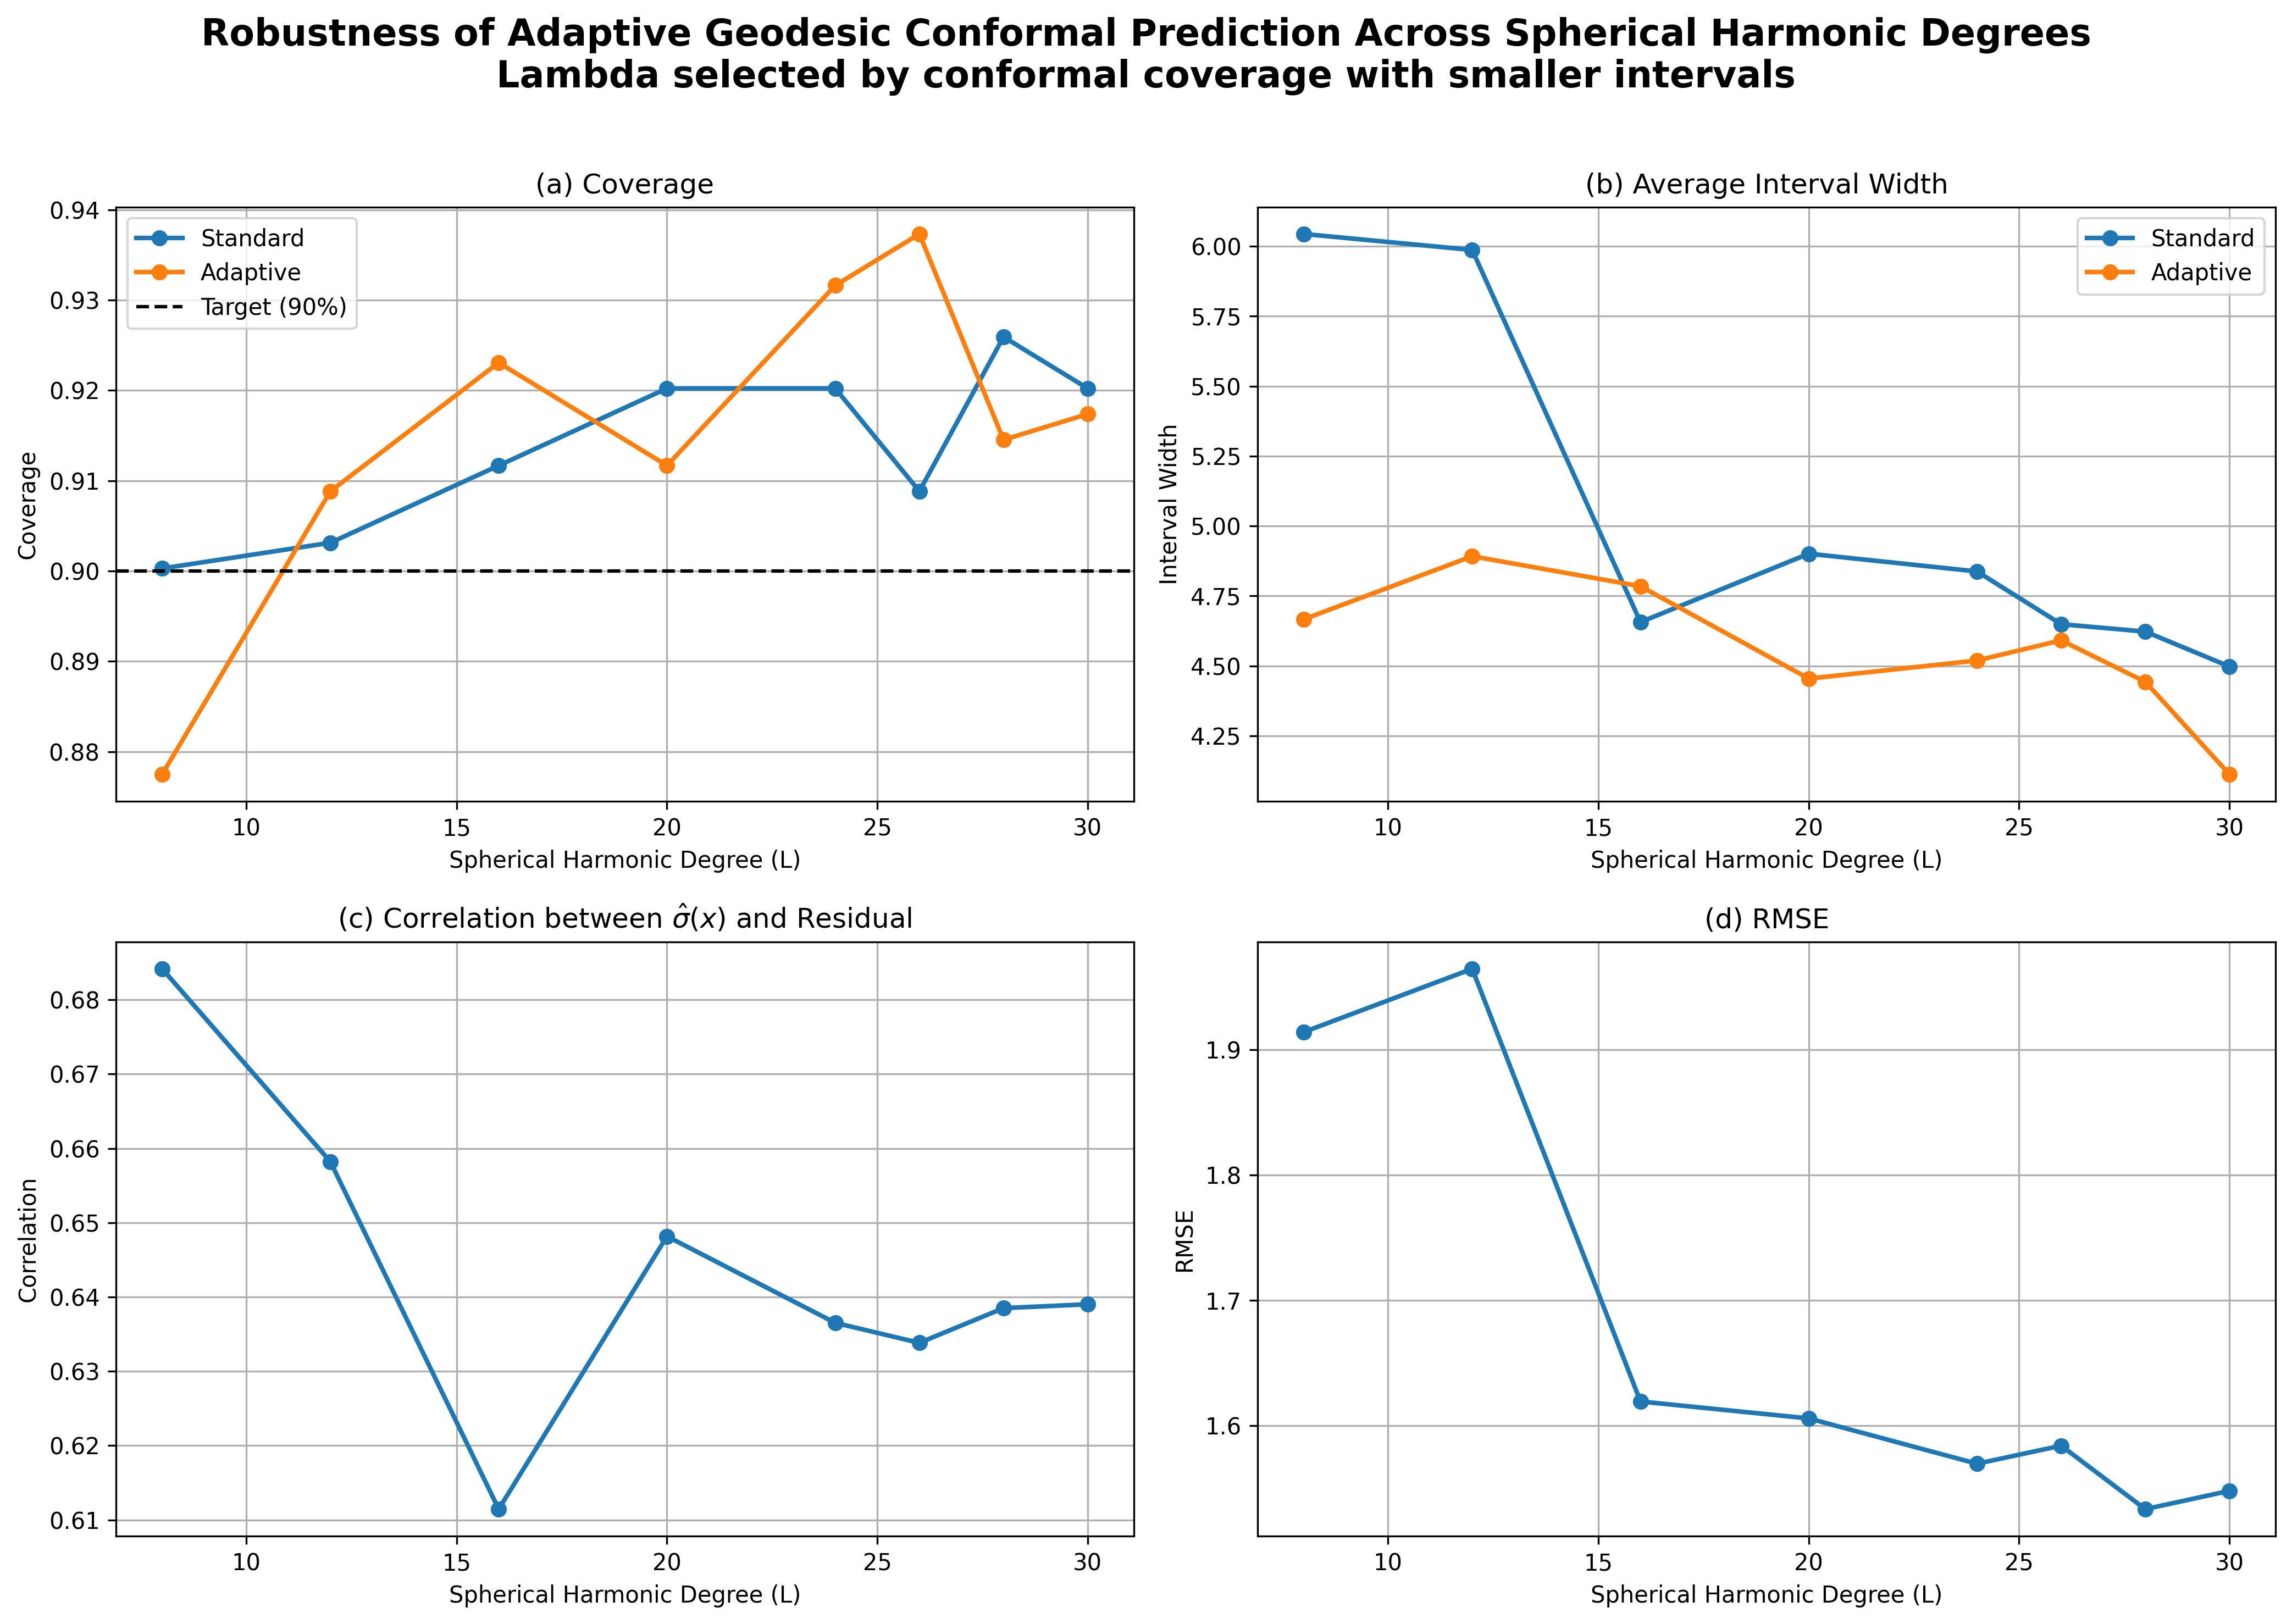
\includegraphics[width=\textwidth]{figures/degree_robustness_conformal_lambda_summary.png}
    \caption{Robustness of adaptive geodesic conformal prediction across spherical harmonic degree $L$, with $\lambda$ selected to minimise adaptive interval width subject to a $90\%$ validation-coverage constraint. (a) Coverage. (b) Mean interval width. (c) Correlation between $\hat\sigma(x)$ and true residual. (d) Test RMSE.}
    \label{fig:degree-robustness}
\end{figure}
To assess whether the main results in  \cref{sec:main-results} depend strongly on the specific degree $L=26$, the full pipeline was repeated for $L\in\{8,12,16,20,24,26,28,30\}$. At each degree, $\lambda$ is re-selected using both the RMSE-minimising and conformal-efficiency criteria described in \cref{ch:methodology}. \Cref{fig:degree-robustness} shows the results for the conformal-selected $\lambda$. Adaptive coverage (panel (a)) stays reasonably close to the $90\%$ target across the tested degrees, while adaptive interval width (panel (b)) is generally similar or below the standard interval width, except for $L\geq20$, which suggests that adaptive uncertainty does not require substantially wider intervals at higher levels of model complexity. The difficulty-estimator correlation $r$ (panel (c)) is highest at the lowest degree tested ($r=0.684$ at $L=8$) and settles into a relatively stable range of approximately $0.63$-$0.66$ for $L\geq20$, suggesting that the relationship between estimated difficulty and actual prediction error remains reasonably stable across higher model degrees. Test RMSE (panel (d)) shows an overall decrease as the degree increases, with only a small increase from $L=8$ to $L=12$, before decreasing substantially from $L=12$ to $L=16$ and then slowly decreasing towards $L=30$. The results suggest that the improvements become smaller and somewhat non-monotonic beyond $L=24$, indicating a gradual reduction in the benefit of additional model complexity. Overall, the adaptive conformal method remains reasonably stable across different spherical harmonic degrees. Increasing model complexity generally improves reconstruction accuracy, but the benefit becomes smaller at higher degrees. The uncertainty results do not appear to depend strongly on selecting exactly $L=26$. This provides evidence of robustness to the choice of spherical harmonic model complexity.
\begin{table}[H]
\centering
\caption{Degree-robustness results with $\lambda$ selected by conformal efficiency (minimum adaptive width subject to $\ge 90\%$ validation coverage). ``Std.\ cov.'' / ``Adapt.\ cov.'' are test-set marginal coverage; $r$ is the difficulty-estimator correlation; $\sigma_{\mathrm{cond}}$ is the six-bin conditional coverage standard deviation; ``Worst'' is the worst-bin coverage.}
\label{tab:degree-robustness}

\resizebox{\textwidth}{!}{%
\begin{tabular}{lccccccccc}
\toprule
$L$ & $\lambda$ & Std.\ cov. & Adapt.\ cov. & Std.\ width & Adapt.\ width & $r$ & $\sigma_{\mathrm{cond}}$ & Worst & RMSE \\
\midrule
8  & $3.16\times10^{-6}$ & 0.900 & 0.877 & 6.044 & 4.667 & 0.684 & 0.036 & 0.828 & 1.914 \\
12 & $1.00\times10^{-2}$ & 0.903 & 0.909 & 5.987 & 4.892 & 0.658 & 0.043 & 0.867 & 1.965 \\
16 & $1.00\times10^{-6}$ & 0.912 & 0.923 & 4.657 & 4.785 & 0.611 & 0.034 & 0.891 & 1.619 \\
20 & $1.00\times10^{-4}$ & 0.920 & 0.912 & 4.901 & 4.455 & 0.648 & 0.036 & 0.864 & 1.606 \\
24 & $3.16\times10^{-5}$ & 0.920 & 0.932 & 4.838 & 4.520 & 0.637 & 0.034 & 0.897 & 1.570 \\
26 & $1.00\times10^{-4}$ & 0.909 & 0.937 & 4.649 & 4.592 & 0.634 & 0.044 & 0.881 & 1.584 \\
28 & $3.16\times10^{-4}$ & 0.926 & 0.915 & 4.623 & 4.443 & 0.638 & 0.044 & 0.847 & 1.533 \\
30 & $3.16\times10^{-5}$ & 0.920 & 0.917 & 4.498 & 4.113 & 0.639 & 0.051 & 0.852 & 1.548 \\
\bottomrule
\end{tabular}%
}
\end{table}
\Cref{tab:degree-robustness}  lists the detailed results for the conformal-selected $\lambda$ at each spherical harmonic degree, including the six-bin conditional-coverage standard deviation and worst-bin coverage. The conditional coverage standard deviation remains within $0.033$ to $0.051$ across all tested degrees, whereas the worst-bin coverage ranges from $0.828$ to $0.897$. Conditional coverage does vary a little across model degrees, yet the overall behaviour remains quite good. These results suggest that the advantage of the adaptive method over the standard baseline in \cref{sec:main-results} at $L=26$ can also be observed across other spherical harmonic degrees.

The marginal-coverage columns of \cref{tab:degree-robustness} assess how stable the conformal calibration is when the model complexity changes. For the eight degrees tested, standard conformal marginal coverage ranges from $90\%$ to $92.6\%$, while adaptive conformal marginal coverage ranges from $87.7\%$ to $93.7\%$. Only at $L=8$ is adaptive coverage slightly below the nominal 90\% target, while at the other tested degrees, it stays reasonably close to $90\%$.  This indicates that the calibration procedure remains broadly stable as the spherical harmonic degree changes, with some variation expected because of finite test/calibration sample sizes.

The test RMSE from 1.914 at $L=8$ drops to approximately 1.53-1.55 for $L=28$, indicating that the accuracy of the base model improves. However, the improvement becomes smaller when the degree becomes higher, which suggests a diminishing benefit from adding further model complexity. Also, the correlation and conditional coverage remain relatively stable across all tested degrees. So, the main findings are not strongly affected by the choice of $L$.
\begin{figure}[H]
    \centering
    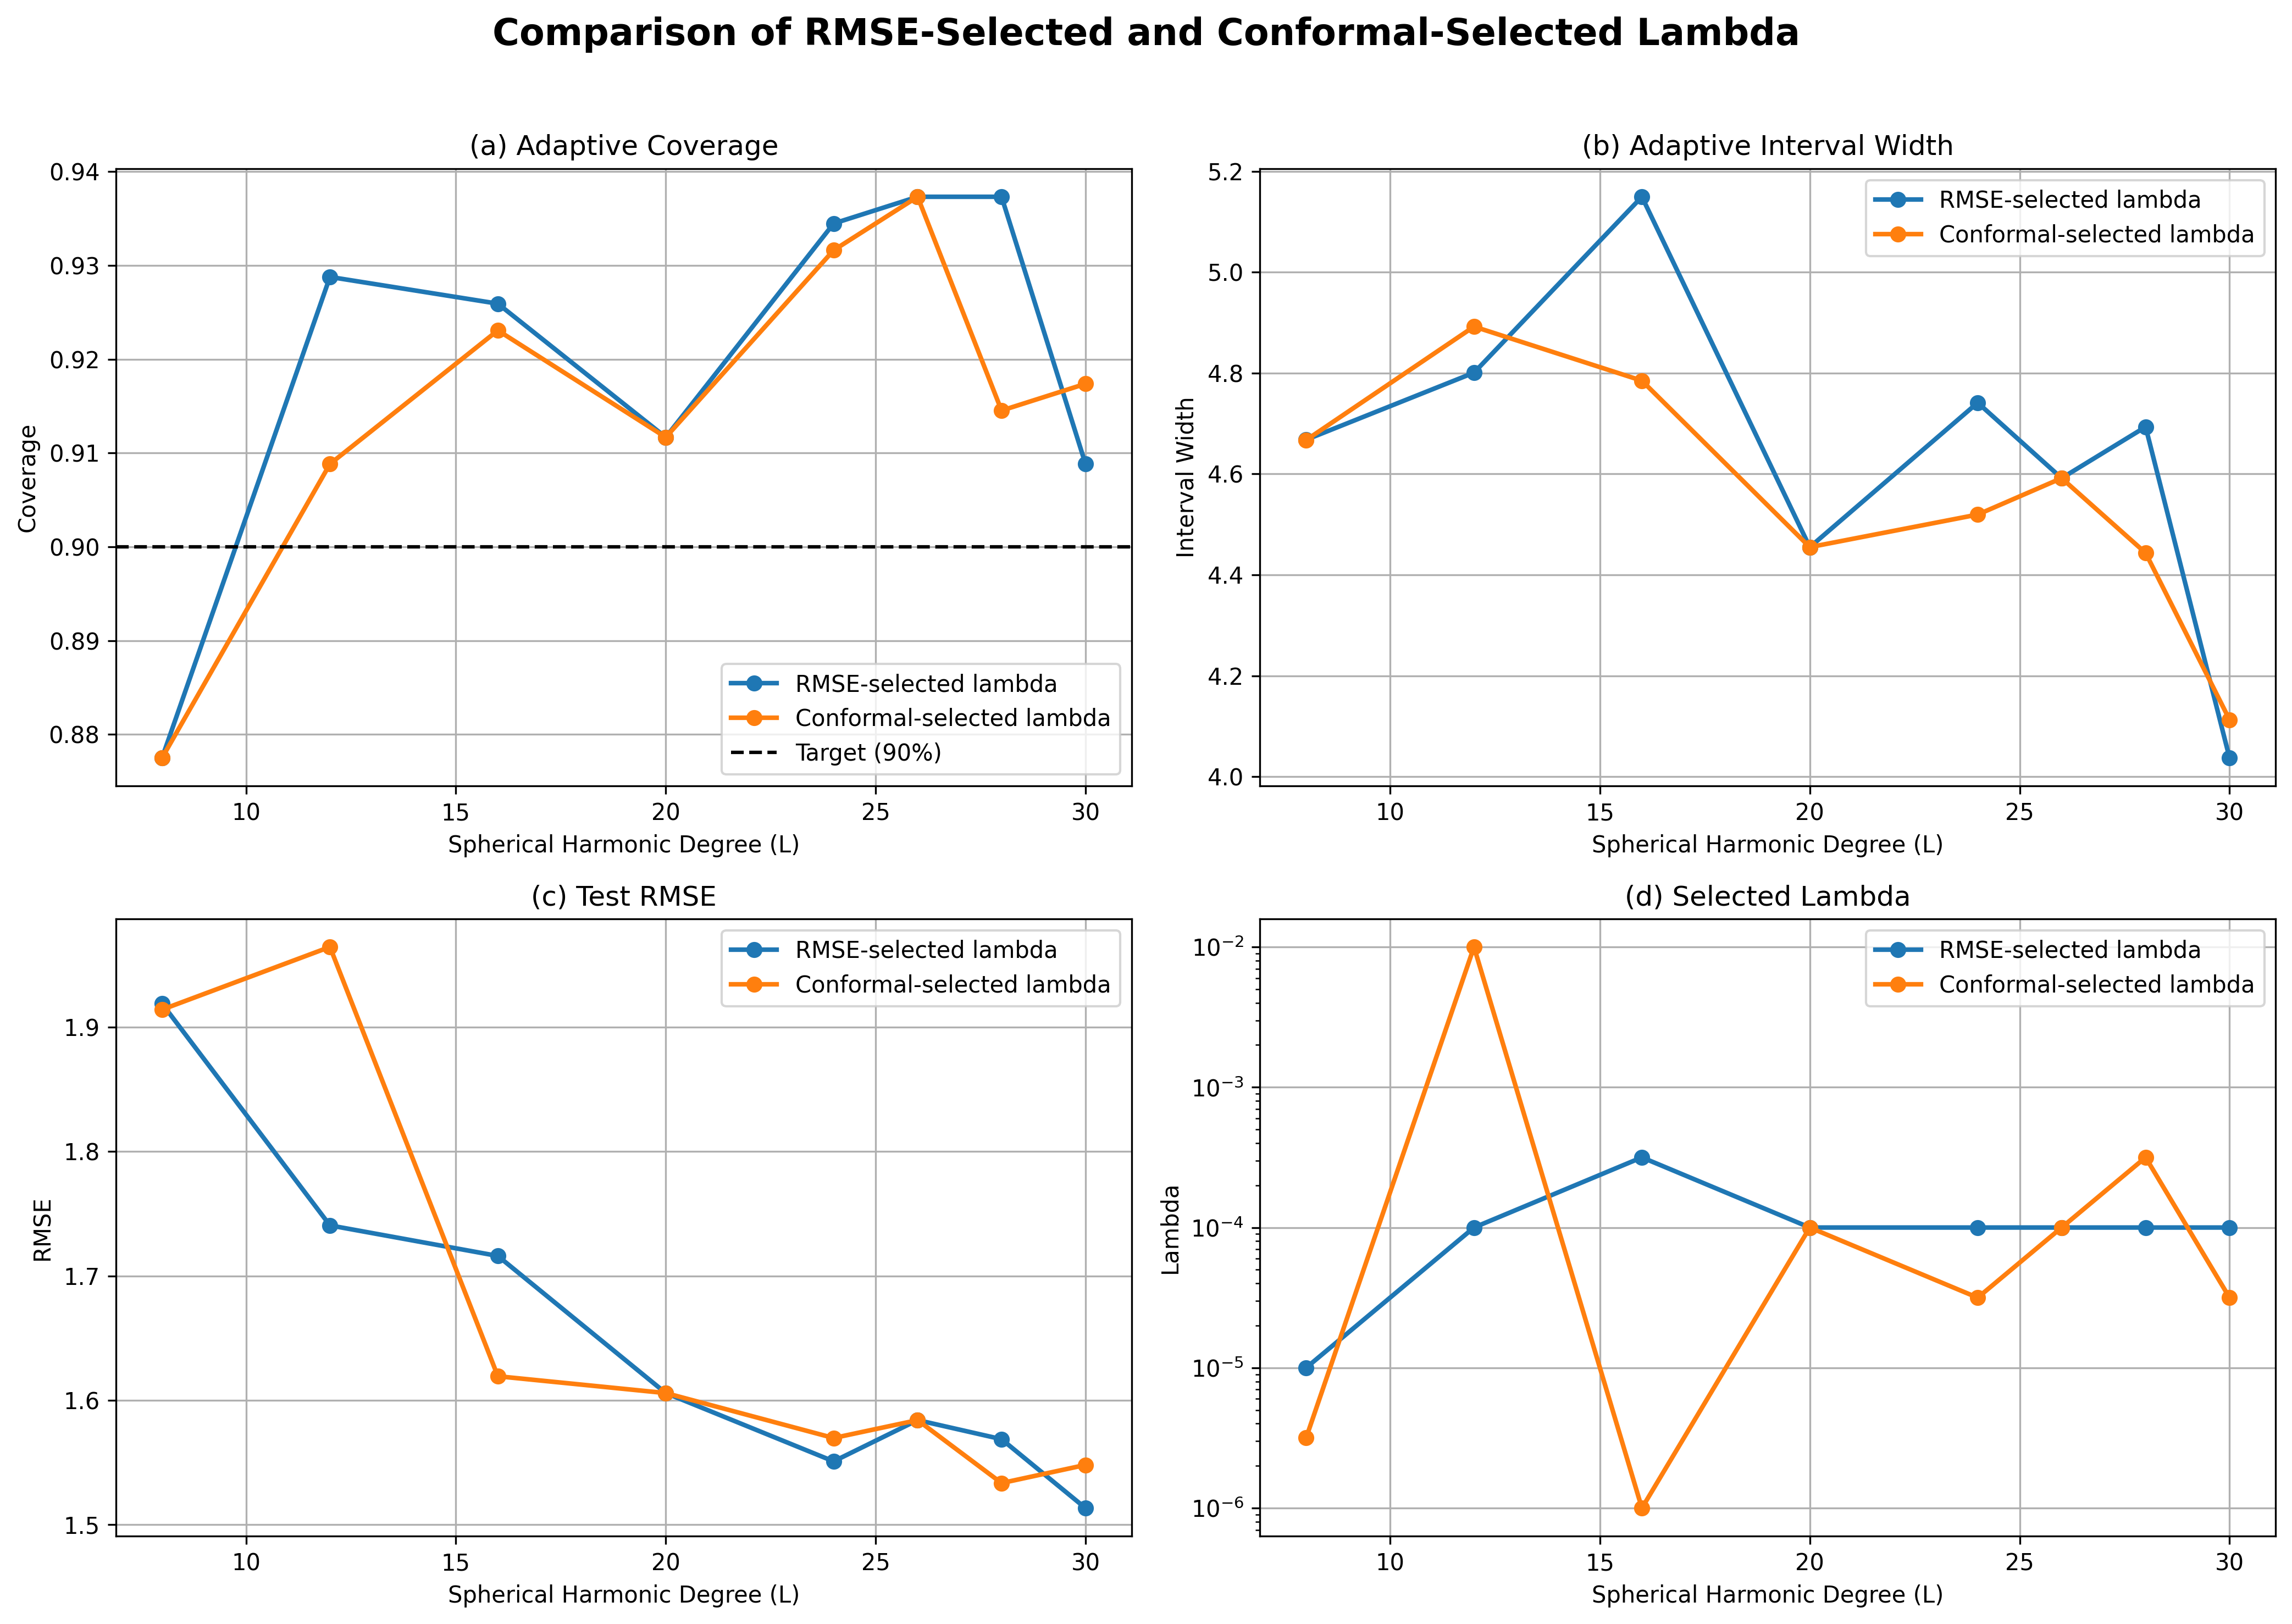
\includegraphics[width=\textwidth]{figures/degree_robustness_lambda_comparison_summary.png}
    \caption{Comparison of RMSE-selected and conformal-efficiency-selected regularisation strength $\lambda$ across spherical harmonic degree.}
    \label{fig:lambda-comparison}
\end{figure}
\Cref{fig:lambda-comparison} compares two different criteria for selecting $\lambda$: RMSE-based selection, which prioritises prediction accuracy, and conformal-based selection, which prioritises interval efficiency while satisfying the coverage requirement. Overall, both methods are consistent in direction for adaptive coverage, interval width, and test RMSE except for the $\lambda$ results in panel (d). For example, at $L=12$, the RMSE-selected $\lambda=10^{-4}$, while the conformal-selected $\lambda=10^{-2}$. This suggests that changing the selection criterion does not appear to cause a large change in overall performance, but the selected $\lambda$ changes depending on the objective being prioritised. Prediction accuracy and conformal interval efficiency appear to be positively correlated in this experiment. However, this should be treated as an empirical observation but not a theoretical guarantee. The two criteria focus on different objectives. A $\lambda$ value that gives the lowest RMSE may not produce the narrowest conformal intervals while still maintaining the required coverage. Therefore, the similar results observed here do not mean that the two selection approaches will always produce the same results.

\section{Full-field reconstruction and geographic uncertainty}
\label{sec:geography}
\begin{figure}[H]
    \centering
    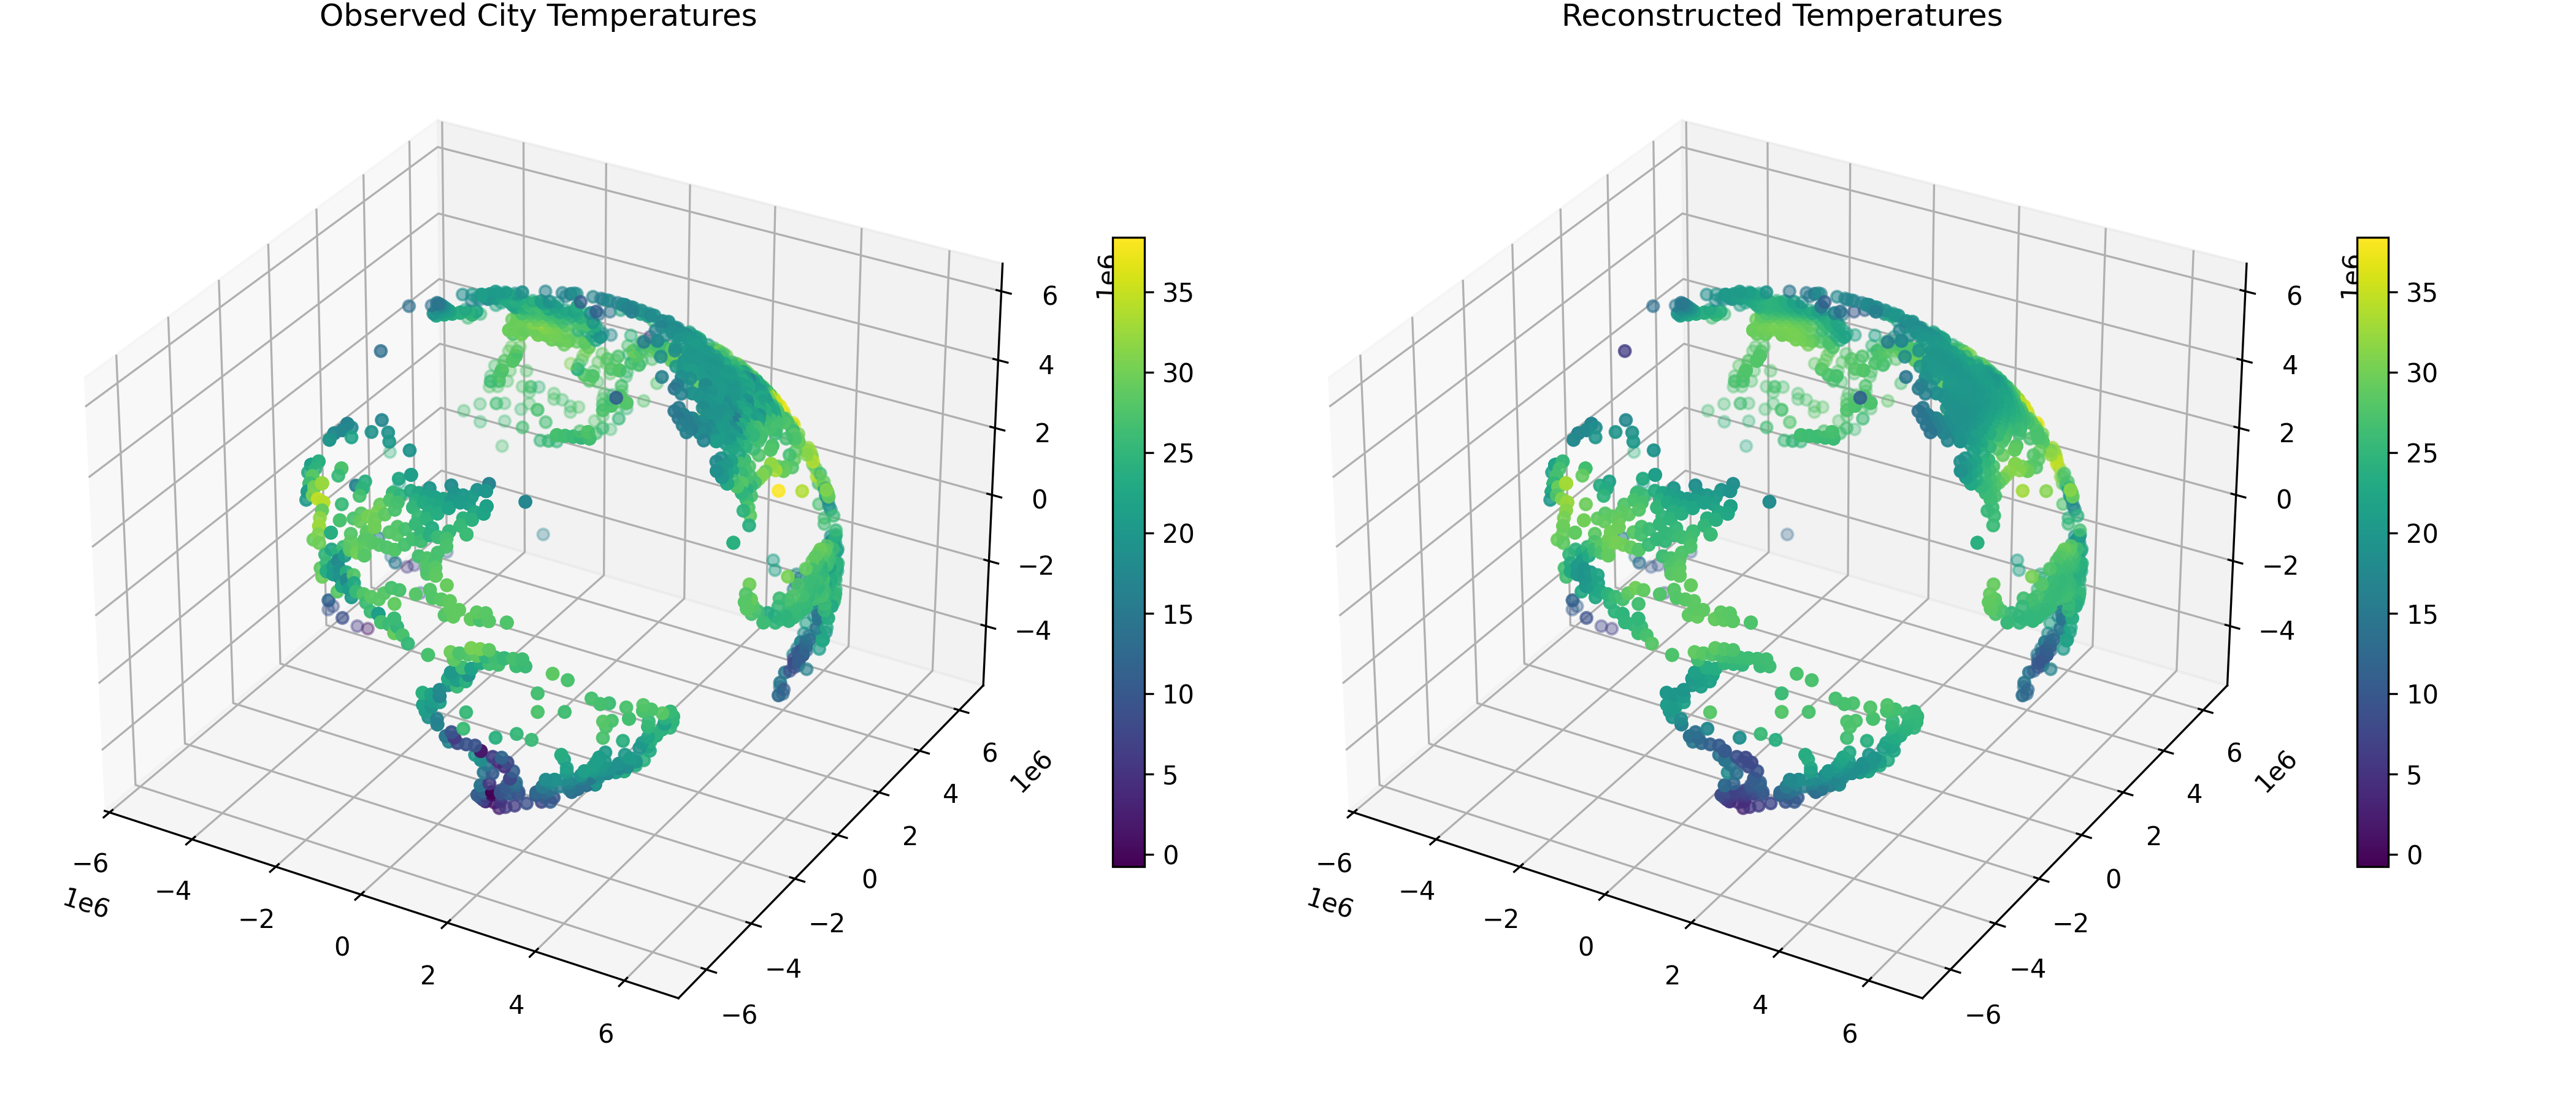
\includegraphics[width=\textwidth]{figures/observed_vs_reconstructed.png}
    \caption{Observed (left) and reconstructed (right) city temperatures, plotted on a 3D globe of Earth's radius. Both use the same colour scale.}
    \label{fig:reconstructed}
\end{figure}
The calibrated model ($L=26$, $\lambda=10^{-4}$, $k=2$) is used to reconstruct the temperature field on a dense $50\times50$ evaluation grid covering the whole sphere. It is also evaluated separately at all $3{,}510$ city locations, giving an overall reconstruction $\mathrm{RMSE}=1.442^\circ\mathrm{C}$, $\mathrm{MAE}=0.921^\circ\mathrm{C}$, and bias $-0.004^\circ\mathrm{C}$. These values indicate the reconstructed temperatures are generally close to the observed temperatures. The evaluation includes training points, and thus it reflects the overall reconstruction fit. They should not be interpreted as out-of-sample performance. The out-of-sample accuracy is evaluated separately using the held-out test set in \cref{sec:main-results}. \Cref{fig:reconstructed} compares the observed and reconstructed temperature fields. The reconstruction captures the main latitudinal patterns and the continental patterns in the observed data. This suggests that the spherical harmonic model successfully captures the large-scale structure of the observed temperature field.
\begin{figure}[H]
    \centering
    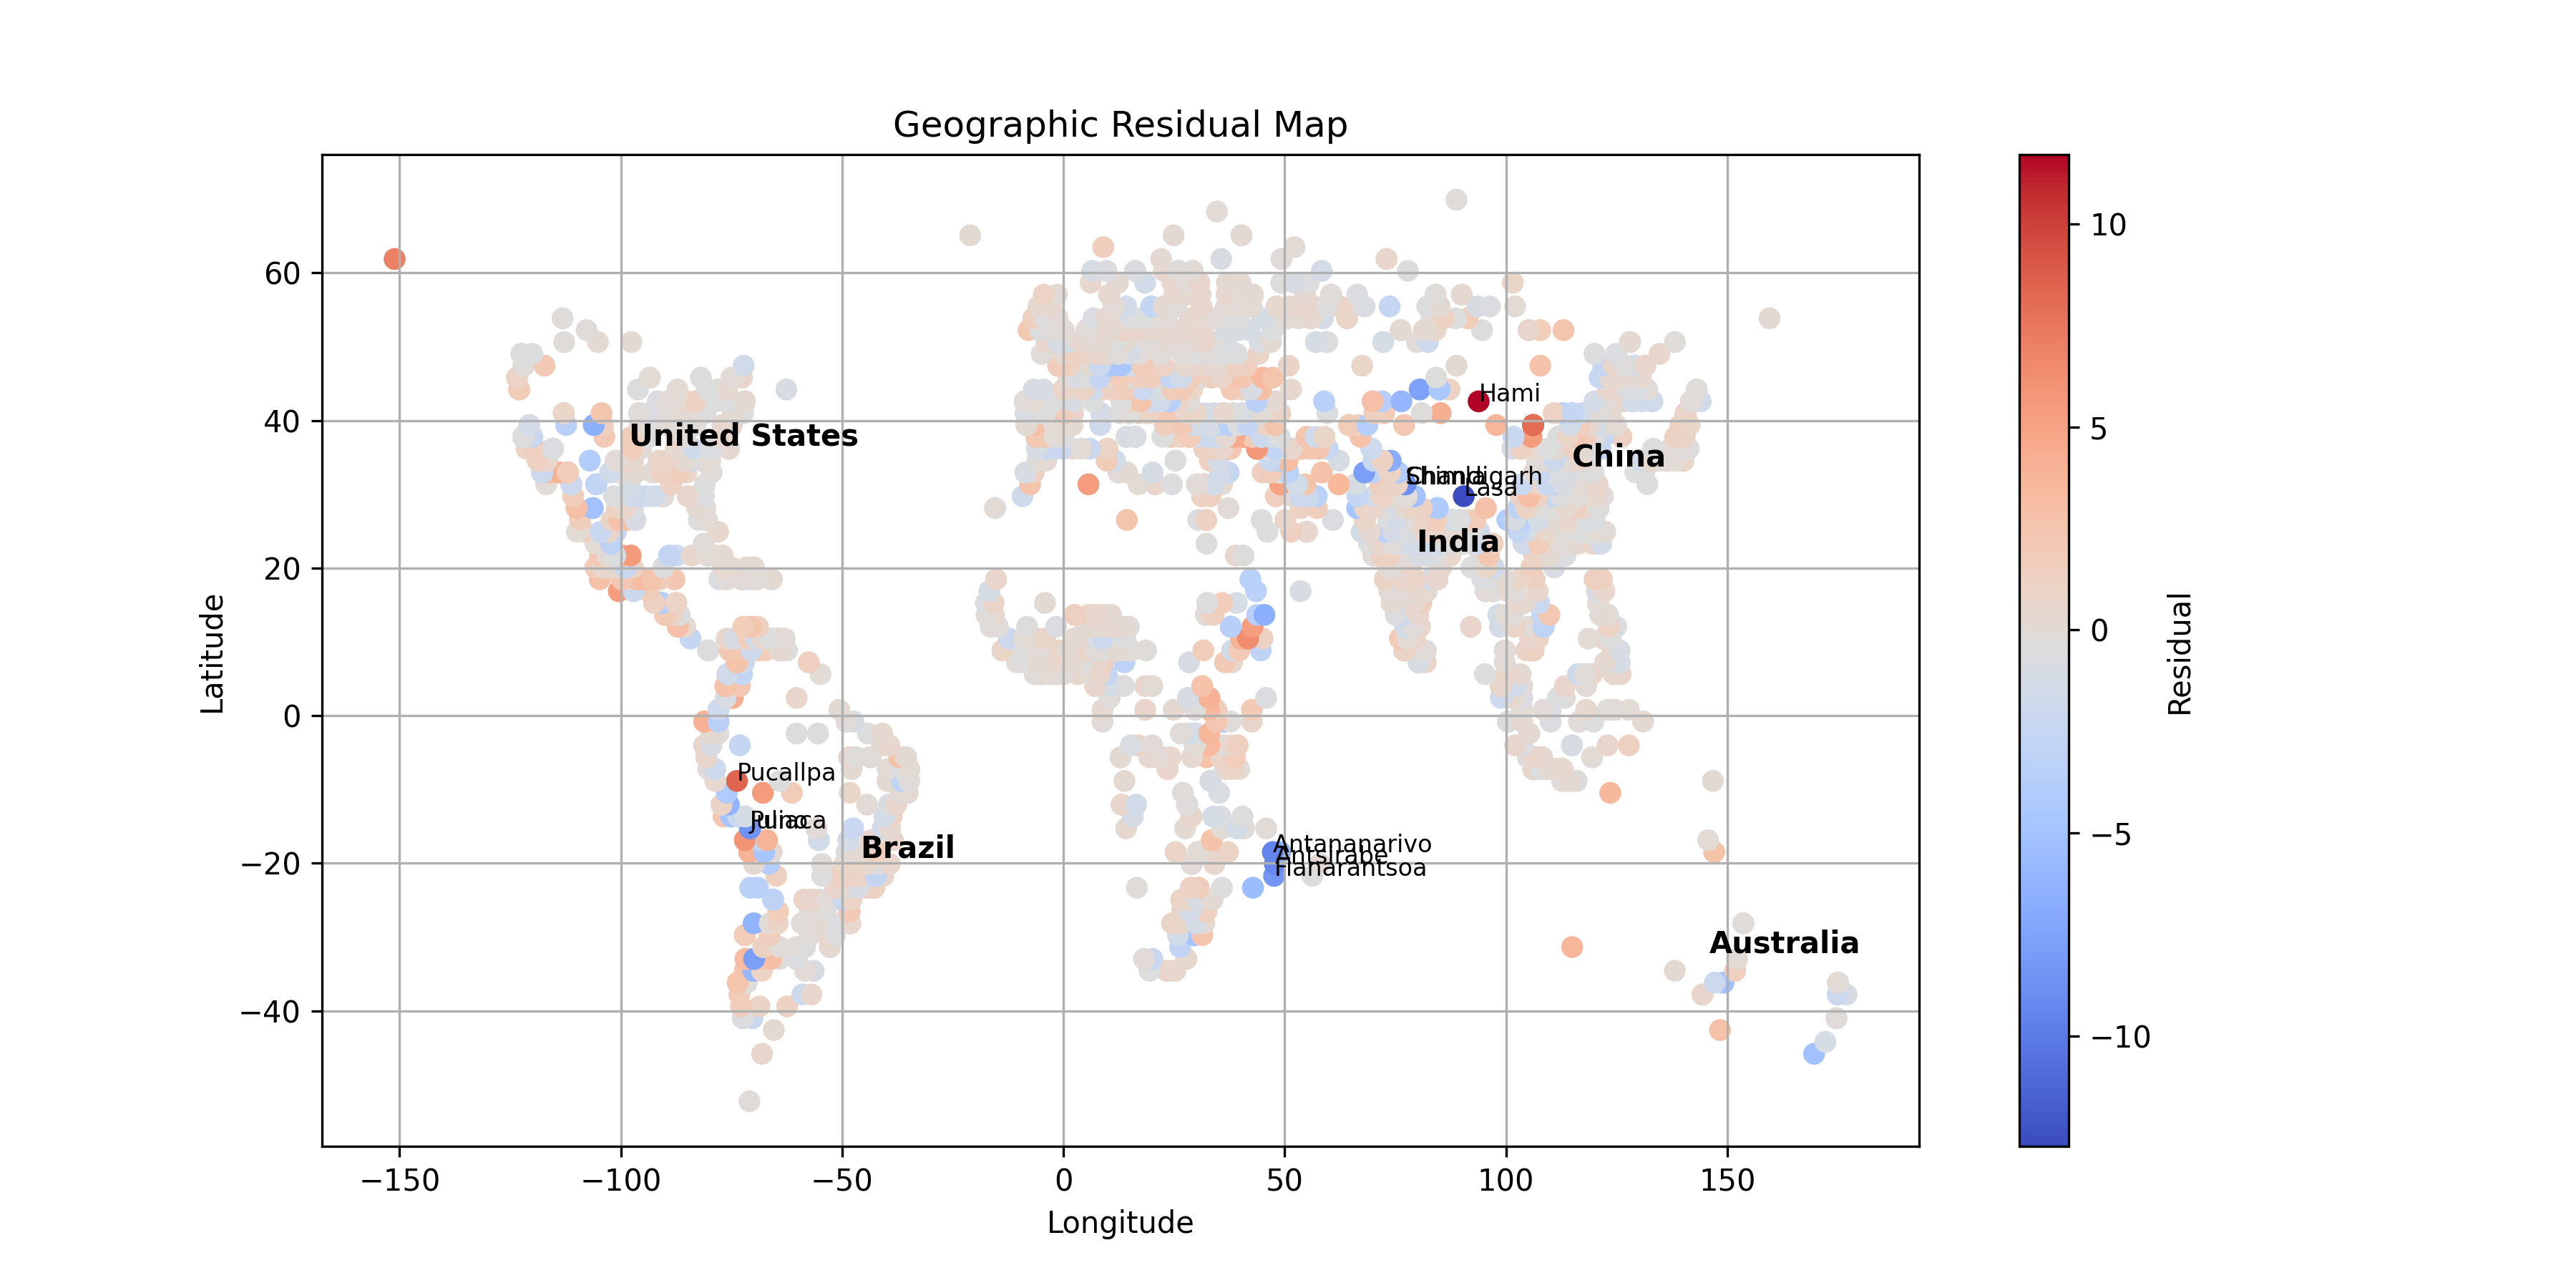
\includegraphics[width=\textwidth]{figures/geographic_residual_map.png}
    \caption{Geographic distribution of signed reconstruction residuals (observed minus predicted), with the ten largest-magnitude residual cities and several major-country centroids labelled for orientation.}
    \label{fig:geo-residual}
\end{figure}
The residual field (\cref{fig:geo-residual}) shows the geographic distribution of reconstruction residuals. No obvious large-scale systematic geographic pattern is observed here, and the residuals are relatively small for most locations. The overall reconstruction bias reported above ($-0.004^\circ\mathrm{C}$) is negligible relative to the overall variation in global city temperatures. However, a small number of cities have noticeably larger residuals in both directions. For instance, Hami, China, is over-predicted, while several Himalayan-region stations are under-predicted. These larger residuals may be related to local climatic characteristics, such as extreme continental conditions, high-altitude environments, or other local effects. These local variations may be difficult for a smooth spherical harmonic model to represent accurately. At $L=26$, the nominal angular scale associated with the maximum degree is approximately $180^\circ/L \approx 7^\circ$, limiting the model's ability to represent highly localised spatial variation. This might be one reason for some of the larger local residuals.
\begin{figure}[H]
    \centering
    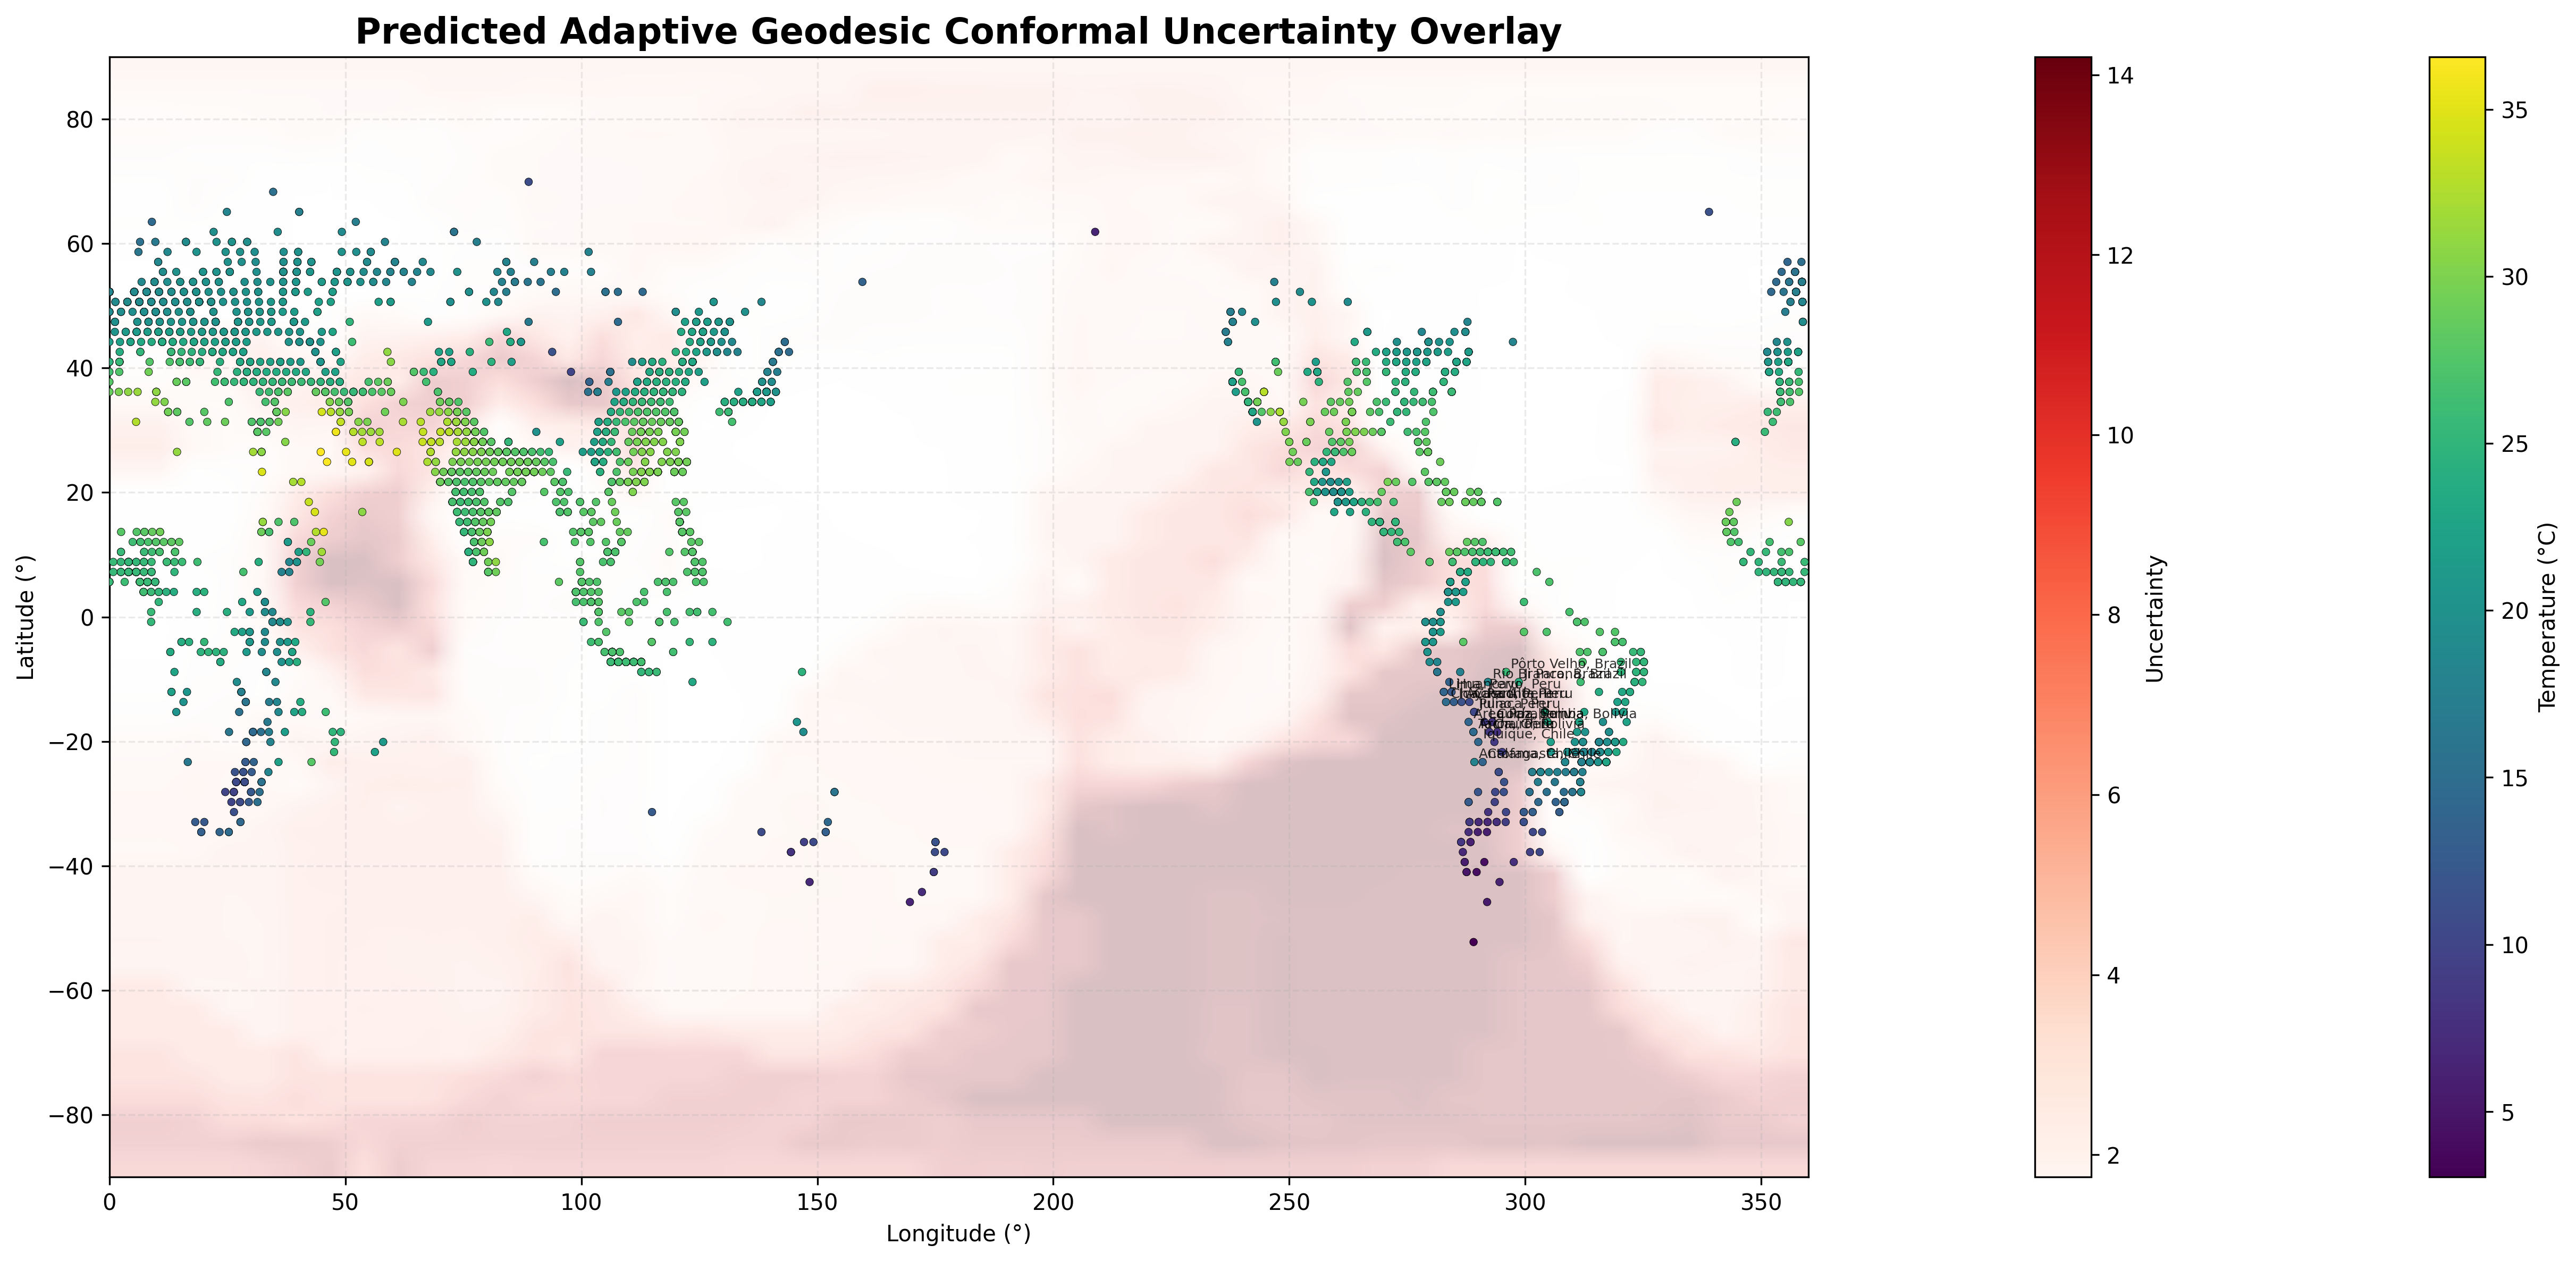
\includegraphics[width=\textwidth]{figures/opened_globe_uncertainty.png}
    \caption{Adaptive geodesic conformal uncertainty (red overlay) and predicted temperature (city markers) on an equirectangular (``opened-globe'') projection. Elevated uncertainty is visible in the sparsely-observed high-Andes region of South America, whose highest-uncertainty cities are labelled.}
    \label{fig:opened-globe}
\end{figure}
The main finding from the geographic analysis is related to \textbf{uncertainty}, rather than just the size of the reconstruction residuals. The cities were ranked based on their estimated difficulty $\hat\sigma(x)$, and the top $5\%$ were then examined (\cref{fig:opened-globe}). The full table is listed in \autoref{ch:appendix}. The twenty highest-uncertainty cities in the entire dataset are mostly concentrated in the high-altitude Andean region of Bolivia, Peru and northern Chile (\cref{fig:opened-globe}). Seventeen of the twenty highest-$\hat\sigma$ cities are from this region, including La Paz, Tacna, Arica, Puno, Juliaca, Arequipa, Cochabamba, Cusco, Ayacucho, Ica, Chincha Alta, Antofagasta, Iquique, Calama, Huancayo, Oruro and Chosica. The remaining three (Pôrto Velho, Rio Branco, Ji-Paraná) are located in the sparsely observed western Brazilian Amazon. Local observation density was also examined to understand the uncertainty results. This includes the number of other cities within $250$, $500$, and $1{,}000,\mathrm{km}$ and the great-circle distance to the $20$th-nearest city. The results show that the high-uncertainty Andean cities generally have only around 2-5 nearby cities within 250 km, while distances of approximately 800--1,400 km are needed to find 20 neighbouring cities. This indicates that these areas have much lower observation density compared with regions such as Europe, eastern China, and the eastern United States. The spatial sparsity provides evidence that limited local observations may contribute to higher estimated uncertainty. Fewer nearby observations mean less local information is available to support the reconstruction. For instance, the Andes also combine low observation density with a distinctive climate environment. High elevation can lead to strong temperature differences compared with lower-altitude locations at similar latitudes, which may be difficult for the smooth spherical harmonic model to capture accurately. The model's spatial resolution is mainly controlled by the global spherical harmonic degree $L$. It does not automatically increase the resolution specifically in areas with complex local terrain. Therefore, local geographic and climatic variation may remain difficult to model. The two possible explanations are consistent, with the observed high-uncertainty locations, insufficient local observation density and genuine physical structure that is not fully captured by the model. The adaptive conformal method also identifies these areas as having higher uncertainty, which suggests that the uncertainty estimates contain meaningful geographic information. However, these results do not prove that either mechanism directly causes the higher uncertainty.
% ============================================================
